%\documentclass{article}
%\usepackage{graphicx,subfigure}
%\begin{document}

\begin{figure}[!h]
  \centering
% 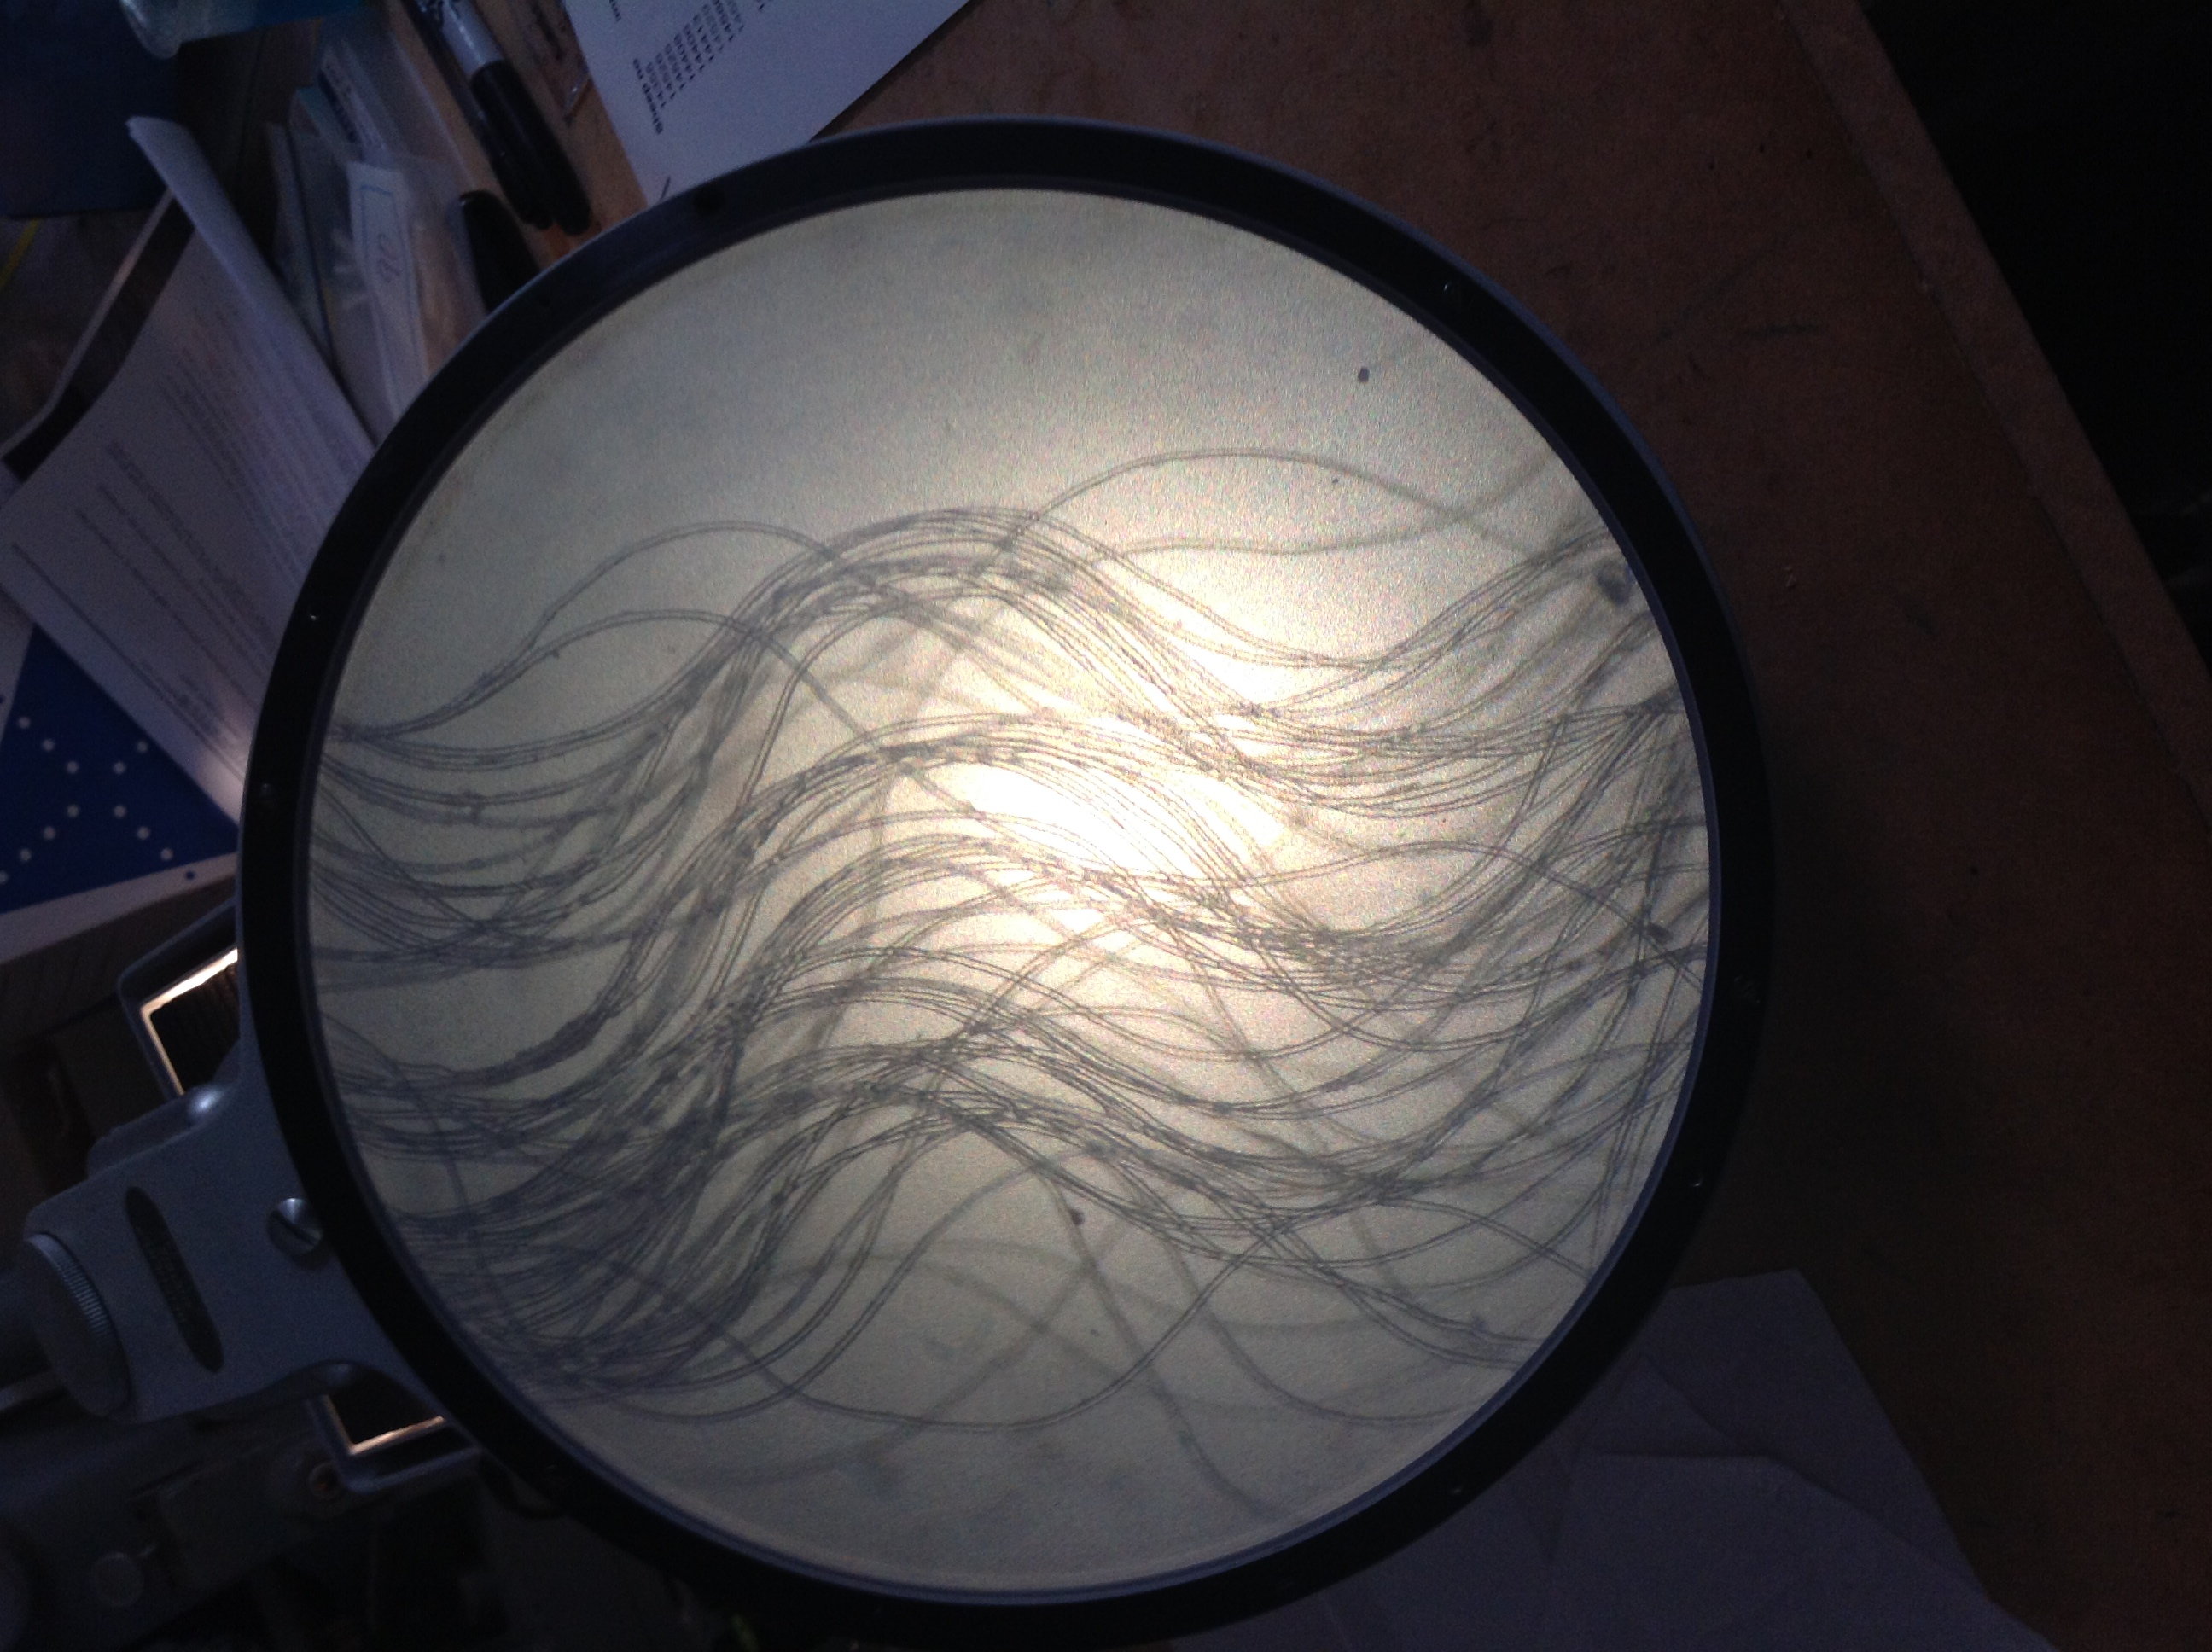
\includegraphics[width=1.0\textwidth]{fignotwist.jpg}
  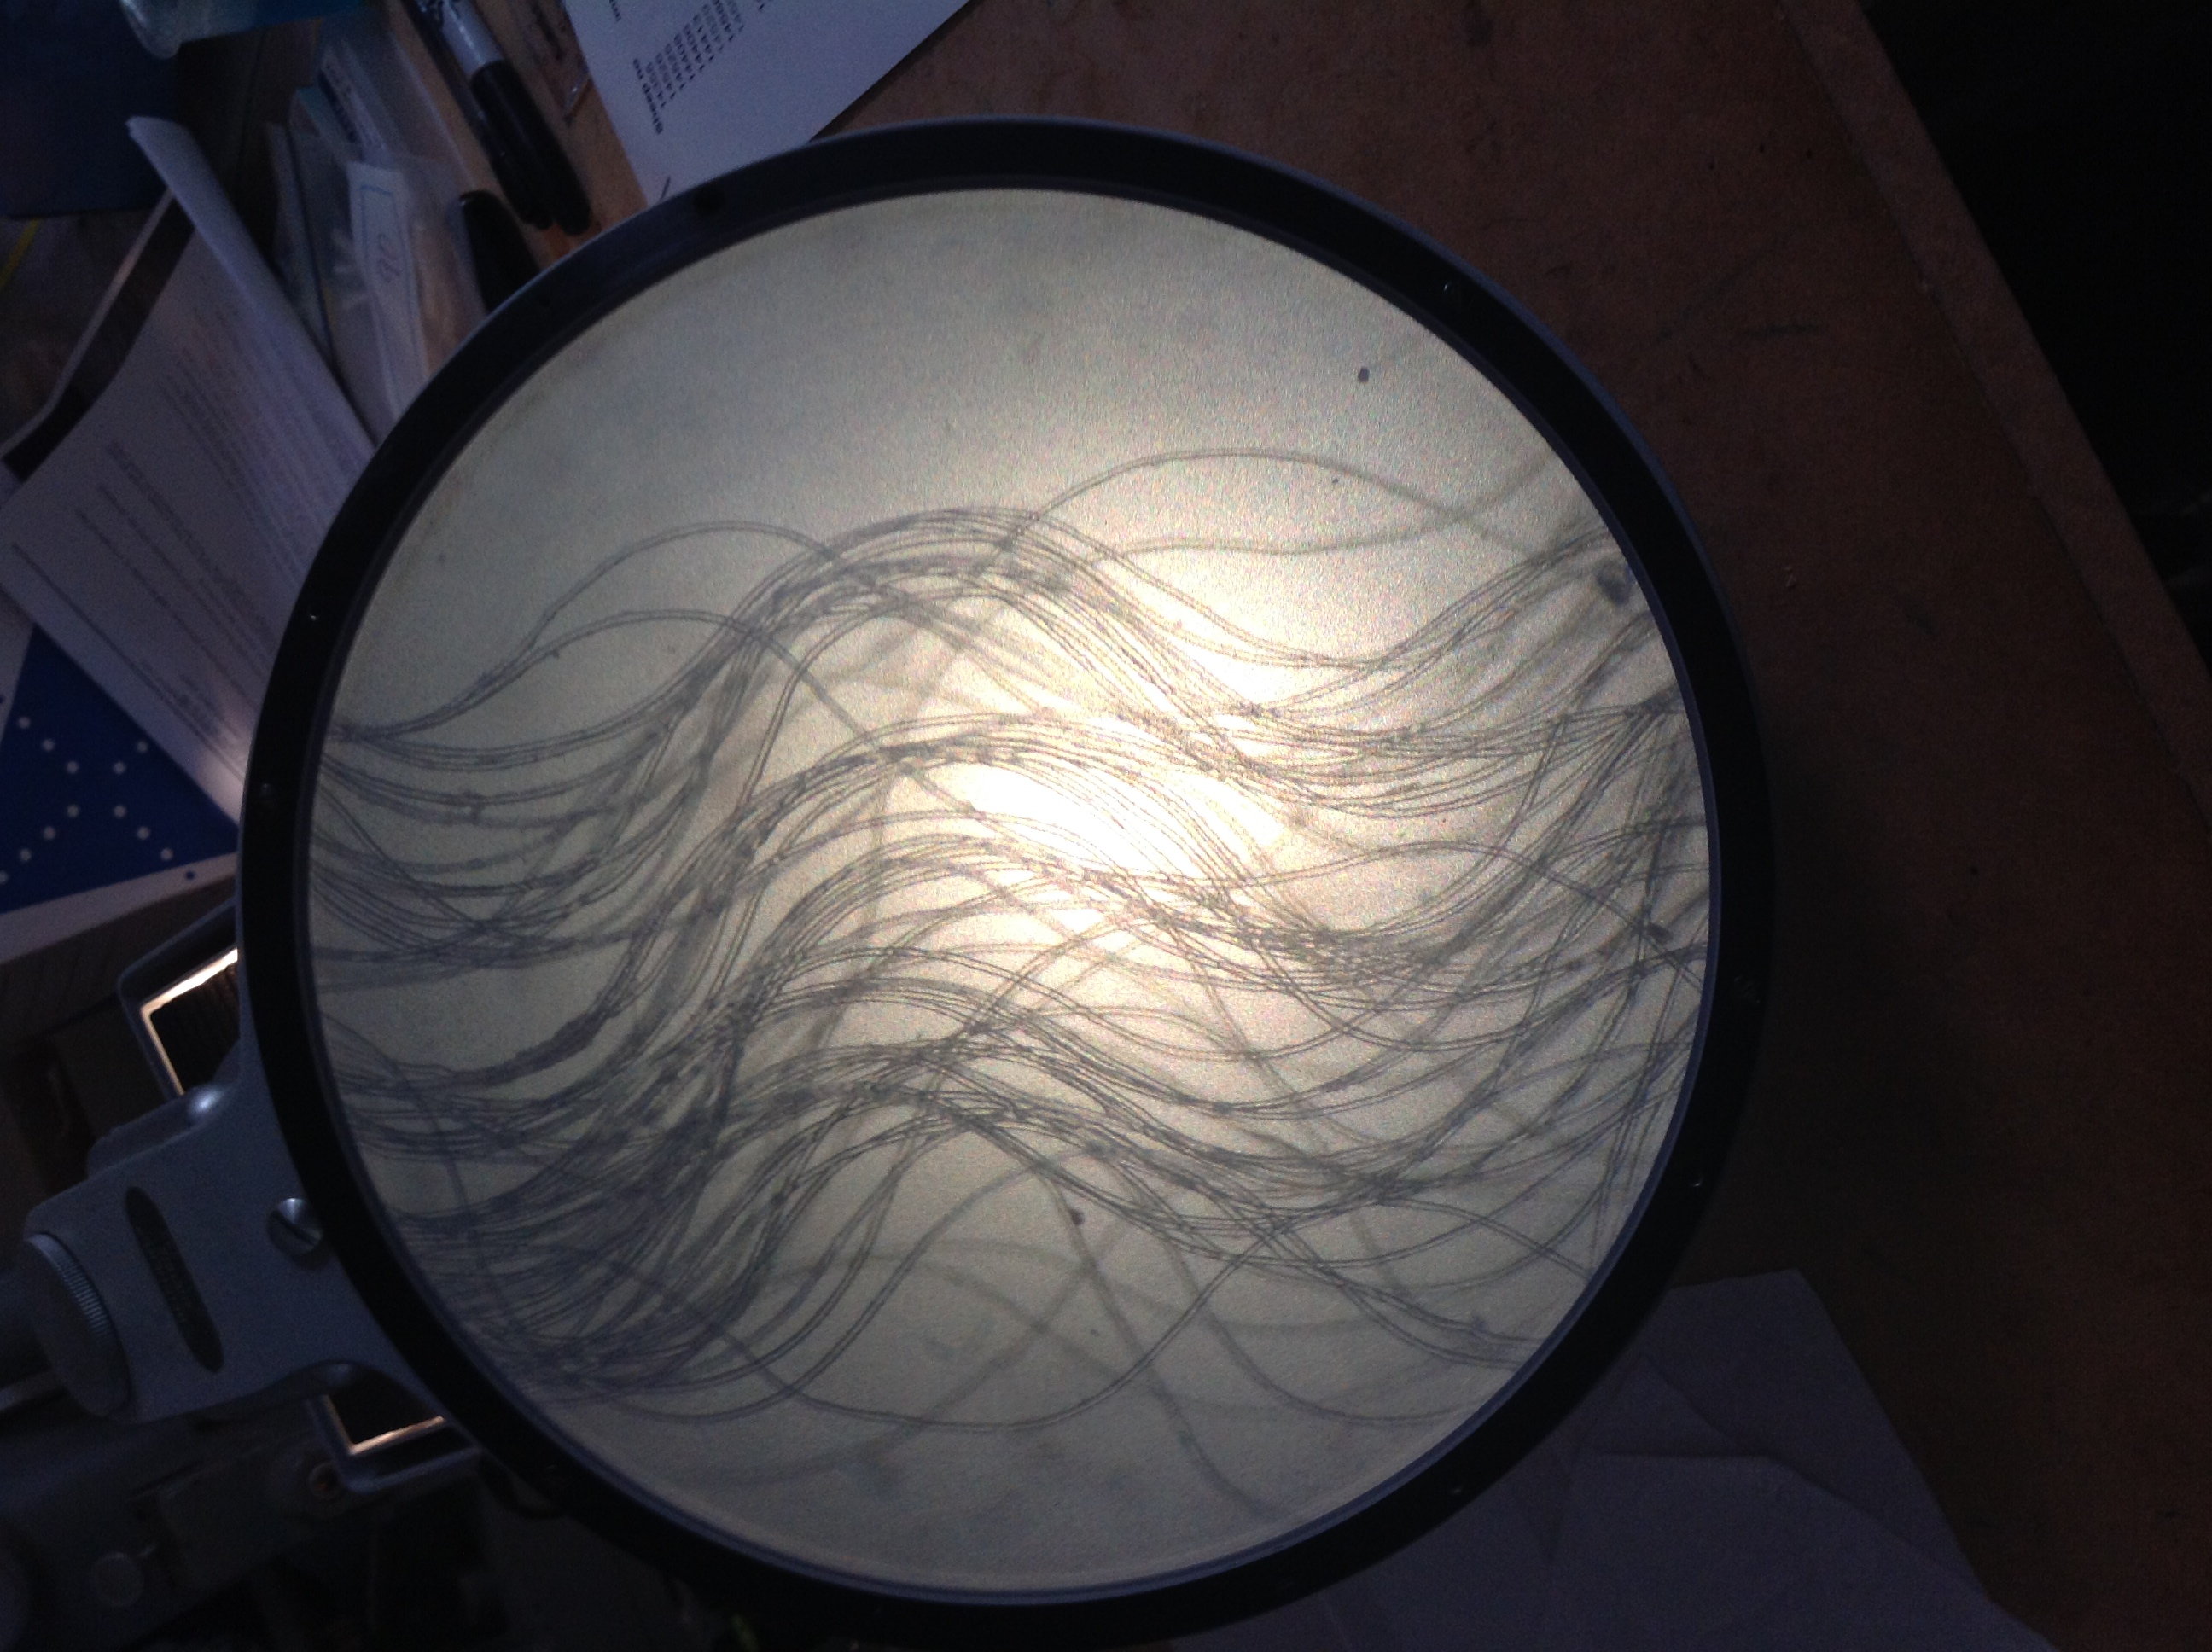
\includegraphics[scale=0.55]{fignotwist.jpg}
%   unalfib516.jpg is original photo on proj mic
  \caption{Photomicrograph, taken with phase contrast microscope, showing a bundle of fibres from a sheep with dished sine wave crimp. Note absence of twisted fibres at any point, and soma unaligned fibres which cross the other fibres at various points. Note sine wave shape of the crimp. Microscope magnification 25x. For printed or screen magnification see Appendix. }
  \label{fig:notwist}
\end{figure}

%\end{document}

